The recurrence to solve is:
$$t(m,n) = t(j,\frac{n}{2}) + a_{m,n} + t(m-j,\frac{n}{2})$$
Where $a_{m,n} = \Theta(mn)$ is the cost of running the algorithm A to find the optimal alignment of sequences of lengths $m$ and $n$.

If we use a notation with weights between zero and one, the recurrence can be written as:
$$t(m,n) = t(\omega_{1,0} m,\frac{n}{2}) + a_{m,n} + t( \omega_{1,1}m,\frac{n}{2})$$
(Where $\omega_{1,1} = 1-\omega_{1,0}$).

We assume for now that $n=2^l$ for some $l$.
\newline
More generally, if we want to unroll all the recursion steps and write the cost of the algorithm, we would need a collection of weights $(\omega_{j,k})_{0 \leq j \leq l , 0 \leq k \leq 2^{j-1} }$, verifying the properties $\omega_{0,0} = 1$, and $\forall j, \forall k, \omega_{j,k} = \omega_{j+1, 2k} + \omega_{j+1, 2k+1}$, so that if we draw a recursion tree, the weight $\omega_{j+1,k}, k in 0,...,2^j$ represents the weight of the node at the $(j+1)^{th}$ recursion level, spawned by the parent node of weight $\omega_{j, \frac{k}{2}  }$.

\begin{figure}[h!]
\begin{center}
   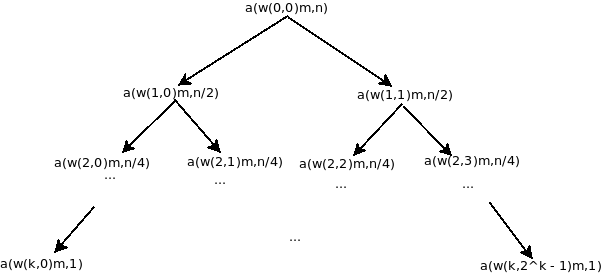
\includegraphics[width=8cm]{recursionTree}
   \caption{Recursion tree with cost of running algorithm A at each node}
\end{center}
\end{figure}

We can see that the sum of all weights at a given recursion depth level is always one, and therefore that the costs $a_{j,k}$ at a given depth level $j$ sum to a $\Theta(m \frac{n}{2^j})$ . That means that at a given recursion depth level (if $m$ and $n$ are big enough), the running cost of the algorithm A is roughly half of the running cost at the previous level.
\newline
\newline
Therefore, the total running time, which is dominated by the sum of the running times of the algorithm A is given by:

\begin{tabular}{lll}
$t(m,n)$ & $ = \sum_{j=0}^{l} {\Theta(m \frac{n}{2^j})}$
\\ & $ = \sum_{j=0}^{l} { \Theta(m 2^j)}$
\end{tabular}


But the serie $\sum_{j=0}^{l} {m 2^j}$ of general term $m 2^j$ is a divergent serie, so that we can write that

\begin{tabular}{lll}
$t(m,n)$  & $ = \Theta( \sum_{j=0}^{l} { m 2^j } )$
\\ & $ = \Theta(mn)$
\end{tabular}

